% test
% Template for PLoS
% Version 3.5 March 2018
%
% % % % % % % % % % % % % % % % % % % % % %
%
% -- IMPORTANT NOTE
%
% This template contains comments intended
% to minimize problems and delays during our production
% process. Please follow the template instructions
% whenever possible.
%
% % % % % % % % % % % % % % % % % % % % % % %
%
% Once your paper is accepted for publication,
% PLEASE REMOVE ALL TRACKED CHANGES in this file
% and leave only the final text of your manuscript.
% PLOS recommends the use of latexdiff to track changes during review, as this will help to maintain a clean tex file.
% Visit https://www.ctan.org/pkg/latexdiff?lang=en for info or contact us at latex@plos.org.
%
%
% There are no restrictions on package use within the LaTeX files except that
% no packages listed in the template may be deleted.
%
% Please do not include colors or graphics in the text.
%
% The manuscript LaTeX source should be contained within a single file (do not use \input, \externaldocument, or similar commands).
%
% % % % % % % % % % % % % % % % % % % % % % %
%
% -- FIGURES AND TABLES
%
% Please include tables/figure captions directly after the paragraph where they are first cited in the text.
%
% DO NOT INCLUDE GRAPHICS IN YOUR MANUSCRIPT
% - Figures should be uploaded separately from your manuscript file.
% - Figures generated using LaTeX should be extracted and removed from the PDF before submission.
% - Figures containing multiple panels/subfigures must be combined into one image file before submission.
% For figure citations, please use "Fig" instead of "Figure".
% See http://journals.plos.org/plosone/s/figures for PLOS figure guidelines.
%
% Tables should be cell-based and may not contain:
% - spacing/line breaks within cells to alter layout or alignment
% - do not nest tabular environments (no tabular environments within tabular environments)
% - no graphics or colored text (cell background color/shading OK)
% See http://journals.plos.org/plosone/s/tables for table guidelines.
%
% For tables that exceed the width of the text column, use the adjustwidth environment as illustrated in the example table in text below.
%
% % % % % % % % % % % % % % % % % % % % % % % %
%
% -- EQUATIONS, MATH SYMBOLS, SUBSCRIPTS, AND SUPERSCRIPTS
%
% IMPORTANT
% Below are a few tips to help format your equations and other special characters according to our specifications. For more tips to help reduce the possibility of formatting errors during conversion, please see our LaTeX guidelines at http://journals.plos.org/plosone/s/latex
%
% For inline equations, please be sure to include all portions of an equation in the math environment.  For example, x$^2$ is incorrect; this should be formatted as $x^2$ (or $\mathrm{x}^2$ if the romanized font is desired).
%
% Do not include text that is not math in the math environment. For example, CO2 should be written as CO\textsubscript{2} instead of CO$_2$.
%
% Please add line breaks to long display equations when possible in order to fit size of the column.
%
% For inline equations, please do not include punctuation (commas, etc) within the math environment unless this is part of the equation.
%
% When adding superscript or subscripts outside of brackets/braces, please group using {}.  For example, change "[U(D,E,\gamma)]^2" to "{[U(D,E,\gamma)]}^2".
%
% Do not use \cal for caligraphic font.  Instead, use \mathcal{}
%
% % % % % % % % % % % % % % % % % % % % % % % %
%
% Please contact latex@plos.org with any questions.
%
% % % % % % % % % % % % % % % % % % % % % % % %

\documentclass[10pt,letterpaper]{article}
\usepackage[top=0.85in,left=2.75in,footskip=0.75in]{geometry}

% amsmath and amssymb packages, useful for mathematical formulas and symbols
\usepackage{amsmath,amssymb}

% Use adjustwidth environment to exceed column width (see example table in text)
\usepackage{changepage}

% Use Unicode characters when possible
\usepackage[utf8x]{inputenc}

% textcomp package and marvosym package for additional characters
\usepackage{textcomp,marvosym}

% cite package, to clean up citations in the main text. Do not remove.
\usepackage{cite}

% Use nameref to cite supporting information files (see Supporting Information section for more info)
\usepackage{nameref,hyperref}

% line numbers
\usepackage[right]{lineno}

% ligatures disabled
\usepackage{microtype}
\DisableLigatures[f]{encoding = *, family = * }

% color can be used to apply background shading to table cells only
\usepackage[table]{xcolor}

% array package and thick rules for tables
\usepackage{array}

% create "+" rule type for thick vertical lines
\newcolumntype{+}{!{\vrule width 2pt}}

% create \thickcline for thick horizontal lines of variable length
\newlength\savedwidth
\newcommand\thickcline[1]{%
  \noalign{\global\savedwidth\arrayrulewidth\global\arrayrulewidth 2pt}%
  \cline{#1}%
  \noalign{\vskip\arrayrulewidth}%
  \noalign{\global\arrayrulewidth\savedwidth}%
}

% \thickhline command for thick horizontal lines that span the table
\newcommand\thickhline{\noalign{\global\savedwidth\arrayrulewidth\global\arrayrulewidth 2pt}%
\hline
\noalign{\global\arrayrulewidth\savedwidth}}


% Remove comment for double spacing
%\usepackage{setspace}
%\doublespacing

% Text layout
\raggedright
\setlength{\parindent}{0.5cm}
\textwidth 5.25in
\textheight 8.75in

% Bold the 'Figure #' in the caption and separate it from the title/caption with a period
% Captions will be left justified
\usepackage[aboveskip=1pt,labelfont=bf,labelsep=period,justification=raggedright,singlelinecheck=off]{caption}
\renewcommand{\figurename}{Fig}

% Use the PLoS provided BiBTeX style
\bibliographystyle{plos2015}

% Remove brackets from numbering in List of References
\makeatletter
\renewcommand{\@biblabel}[1]{\quad#1.}
\makeatother



% Header and Footer with logo
\usepackage{lastpage,fancyhdr,graphicx}
\usepackage{epstopdf}
%\pagestyle{myheadings}
\pagestyle{fancy}
\fancyhf{}
%\setlength{\headheight}{27.023pt}
%\lhead{\includegraphics[width=2.0in]{PLOS-submission.eps}}
\rfoot{\thepage/\pageref{LastPage}}
\renewcommand{\headrulewidth}{0pt}
\renewcommand{\footrule}{\hrule height 2pt \vspace{2mm}}
\fancyheadoffset[L]{2.25in}
\fancyfootoffset[L]{2.25in}
\lfoot{\today}

%% Include all macros below

\newcommand{\lorem}{{\bf LOREM}}
\newcommand{\ipsum}{{\bf IPSUM}}

%% END MACROS SECTION


\begin{document}
\vspace*{0.2in}

% Title must be 250 characters or less.
\begin{flushleft}
{\Large
\textbf\newline{Combined panel test positivity is an uncertain predictor of disease probability in multiplex testing with implications for epidemiological estimates and clinical decision making.} % Please use "sentence case" for title and headings (capitalize only the first word in a title (or heading), the first word in a subtitle (or subheading), and any proper nouns).
}
\newline
% Insert author names, affiliations and corresponding author email (do not include titles, positions, or degrees).
\\
Robert Challen\textsuperscript{1,2*},
Anastasia Chatzilena\textsuperscript{1,2},
George Qian\textsuperscript{1,2},
Glenda Oben\textsuperscript{1,2},
Rachel Kwiatkowska\textsuperscript{3,4},
Catherine Hyams\textsuperscript{1},
Adam Finn\textsuperscript{1},
Krasimira Tsaneva-Atanasova\textsuperscript{5},
Leon Danon\textsuperscript{1,2}
\\
\bigskip
\textbf{1} Bristol Vaccine Centre, University of Bristol, Bristol, UK.\\
\textbf{2} Department of Engineering Mathematics, University of Bristol, Bristol, UK.\\
\textbf{3} Population Health Sciences, University of Bristol, UK.\\
\textbf{4} NIHR Health Protection Unit in Behavioural Science and Evaluation, University of Bristol, UK.\\
\textbf{5} Department of Mathematics and Statistics, University of Exeter, UK.\\
\bigskip

% Insert additional author notes using the symbols described below. Insert symbol callouts after author names as necessary.
%
% Remove or comment out the author notes below if they aren't used.
%
% Primary Equal Contribution Note
% \Yinyang These authors contributed equally to this work.

% Additional Equal Contribution Note
% Also use this double-dagger symbol for special authorship notes, such as senior authorship.
% \ddag These authors also contributed equally to this work.

% Current address notes
% \textcurrency Current Address: Dept/Program/Center, Institution Name, City, State, Country % change symbol to "\textcurrency a" if more than one current address note
% \textcurrency b Insert second current address
% \textcurrency c Insert third current address

% Deceased author note
% \dag Deceased

% Group/Consortium Author Note
% \textpilcrow Membership list can be found in the Acknowledgments section.

% Use the asterisk to denote corresponding authorship and provide email address in note below.
* rob.challen@bristol.ac.uk

\end{flushleft}
% Please keep the abstract below 300 words
\section*{Abstract}

Multiplex panel tests identify many individual causes of disease at once, using a set of component tests. In some panels the number of components can be large. If the panel is detecting causative pathogens for a syndrome or disease then we might wish to estimate the burden of that disease by combining the results of the panel, for example pneumococcal pneumonia as caused by individual pneumococcal serotypes.  When we are dealing with multiplex test panels with many components, test error in the individual components of a panel, even when present at very low levels, can cause significant overall error. Uncertainty in the sensitivity and specificity of the individual tests, and statistical fluctuations in the numbers of false positives and false negatives, will cause large uncertainty in the combined estimates of disease prevalence. In many cases this can be a source of significant bias. In this paper we characterise this issue and present novel methods to adjust for this bias and properly represent the uncertainty when interpreting the combined results of multiplex panel tests. As multiplex testing becomes more common in clinical practice the interpretation of large numbers of test results for uncommon events will become difficult, as the risk of false positives increases with the number of tests. 

% When multiple tests are carried out simultaneously that identify distinct disease subtypes, it seems uncontroversial to combine the component results into a panel to detect the disease super-type in an individual, or quantify the burden of disease in the population. However, if the number of disease subtypes tested for is large then it is likely that the pre-test probability of each individual subtype is low. In this situation false positive results for each subtype test create a compound error that depends on sensitivity, specificity and prevalence of each subtype. This causes the combined test positivity to be a biased estimate of the post-test probability of disease, usually leading to significant over estimation. This complicates the interpretation of the combined panel result. In clinical applications, a higher than expected false positive rate for the super-type, could lead to inappropriate management if not correctly interpreted by the clinician. In epidemiological applications it can lead to significant uncertainty when determining the burden of disease. At an epidemiological level correction of this bias is possible through Bayesian and frequentist methods, but requires a rigorous approach to propagate uncertainty, as estimates of sensitivity and specificity for multiplex tests are often not well characterised.

% Please keep the Author Summary between 150 and 200 words
% Use first person. PLOS ONE authors please skip this step.
% Author Summary not valid for PLOS ONE submissions.
% \section*{Author summary}
% In analysing data on pneumococcal serotypes we discovered ...

\linenumbers

% Use "Eq" instead of "Equation" for equation citations.
\section*{Introduction}

Multiplex panel testing is a convenient and rapid diagnostic tool and is increasingly being used in clinical practice to differentiate between viral and bacterial causes of a range of disorders\cite{ramanan2017}. It has also been used in epidemiological studies to identify pneumococcal subtypes targeted by vaccines\cite{bonten2015} or monitor disease spread\cite{henson2023}. Multiplex panel tests identify multiple subtypes of a wide range of disease, caused by different pathogens, or by different subtypes of the same pathogen\cite{ramanan2017}, and may be based on immunological\cite{pride2012,kalina2020} or genetic techniques\cite{mengelle2013,murphy2020,jaaskelainen2006,jansen2011,grondahl1999,hendolin1997}. The number of targets tested for in each multiplex are increasing, but range from a handful, up to 48 different causative agents\cite{henson2023}.

In the schematic in Fig~\ref{fig1}, we distinguish between multiplex testing (subfigures A-D) and other types of multiple testing (subfigures E-G). Subfigures A-D show two component tests which identify each of two subtypes of disease. The disease subtypes are present independently of each other and the disease super-type is present if any of the subtypes is present (B-C). In panel A we see that a false positive in one component, results in a false positive in the combined panel. In subfigure B one subtype is correctly detected, in C the other subtype, and in subfigure D a false positive result for one subtype and a false negative for the other results in an overall result which is correct for the wrong reason. In all subfigures A-D, the combined test result would be interpreted as positive. As described above, this design of test is usually extended to many more than two subtypes to make a multiplex panel.

% Place figure captions after the first paragraph in which they are cited.
\begin{figure}[!h]
\centerline{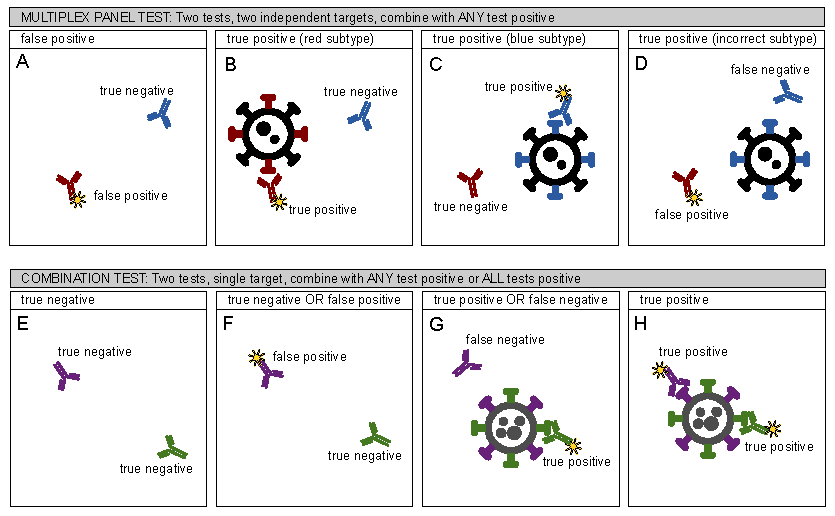
\includegraphics{fig/fig1-testerror-v2.pdf}}
\caption{{\bf Two scenarios for multiple testing.}
Panels A-D depict a multiplex panel test which is the subject of this analysis. It depicts the situation where multiple tests are employed to detect multiple subtypes of disease which may be present separately or together, the results of which are combined to give an overall result, such that if any component test is positive, the combination is positive. An alternative, shown in panels E-H, and not in scope of this paper concerns the situation where multiple tests are used to identify a single condition. In this case two interpretations of the multiple test results are possible, which either maximise test sensitivity or test specificity.}
\label{fig1}
\end{figure}

Subfigures E-H in Fig~\ref{fig1} show a different test design which is more related to multiple modalities of testing\cite{weinstein2005}. In this situation, the multiple tests are looking for the same underlying cause of disease which does not have subtypes. In subfigure E both tests are true negatives and the overall result also a true negative. The interpretation of the two tests can be: a) that any single test being positive infers disease, in which case all subfigures F-H show positive combined results, or b) that both tests must be positive to identify the disease, in which case only subfigure H represents a positive result. These are not regarded as multiplex tests.

In more formal language we define a multiplex test as specifically consisting of a set of independent components which test different independent hypotheses, and the results of which are combined to give a panel result where any positive test result in a component implies a positive test result in the panel. From this point, only multiplex panel tests will be discussed.

If a condition is composed of many subtypes, then each individual subtype must be a fraction of the overall condition prevalence. The more subtypes in a multiplex panel, on average the smaller that fraction will be. If the pre-test probability for each component is low, then each component test is operating at a level where the positive predictive value of the test is also relatively low. This leads to a high probability of observing false positives in each component. We will also observe false negatives depending on the sensitivity of the test, but if the prevalence of a subtype is lower, there are fewer true positives to be missed.

\begin{figure}[hb!]
\centerline{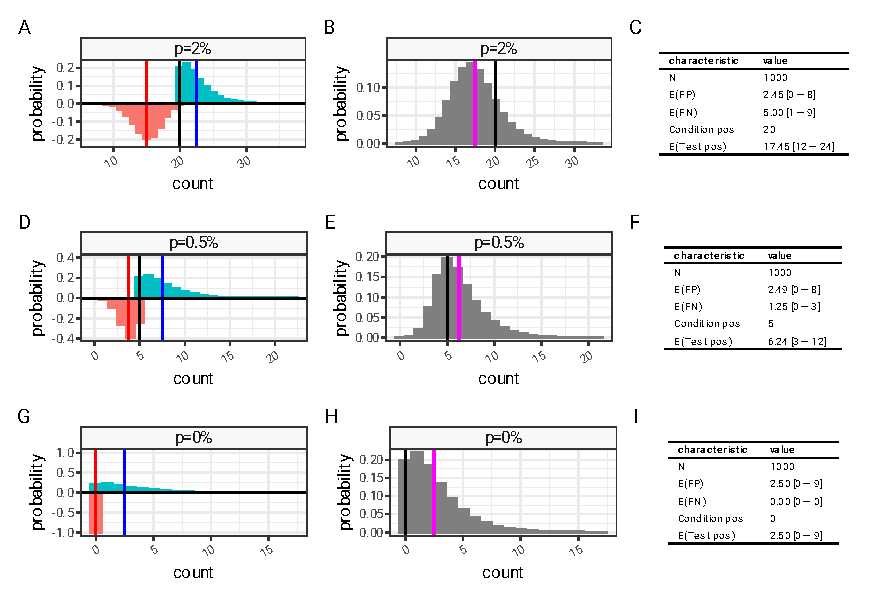
\includegraphics{fig/low-prevalence-sensitivity-specificity.pdf}}
\caption{{\bf Error distributions of test results in low pre-test probability settings.}
Statistical distribution of false positives (cyan bars, with expected value as a blue vertical line) and false negatives (orange bars, expected value red line) of 1000 hypothetical test results with 0.9975 specificity and 0.8 sensitivity at different prevalence levels. Panel A, D and G show the disaggregated distribution of false positives and false negatives and B, E and H the combined error distribution of test positive observations (grey bars), and expected test positivity (magenta line) compared to the true condition positives (black line).}
\label{fig2}
\end{figure}

The effect of this can be seen in Fig~\ref{fig2} where we look at the theoretical distribution of false negatives and false positives in 1000 tests for three hypothetical disease subtypes, present at 2\%, 0.5\% and 0\% prevalence, assuming a test with high specificity of 99.75\% and moderate sensitivity of 80\%. At 2\% prevalence false positive test results are likely to be balanced by the false negatives, subfigure A, and the expected test positivity is expected to be lower than 2\%, the true value of prevalence in this simulation, (subfigure B and C). When the prevalence of the subtype is lower at 0.5\% this pattern is reversed and the false positives will tend to outweigh the false negatives (D) leading to a higher test positivity than prevalence (E and F). In the 0\% scenario in (G,H and I) all positives are by definition false positives, and distributed with high variance.

If a multiplex panel which consists of 20 subtypes, is applied to a disease which is present at a prevalence of 10\%, then it is reasonable to expect that the three patterns in Fig~\ref{fig2} will be present in some combination. The components have a mix of false positives and false negatives, in a manner dependant on the distribution of disease subtypes. In this particular scenario (20 highly specific tests at 10\% prevalence) the balance of these will be towards false positives. Because any positive component results in a positive panel result, the component false positive errors compound in combination. In this example the error combines in such a way that the panel result will contain more false positives than false negatives, and the resulting test positivity rate will be an overestimate of true prevalence.

% The compounding of error in numerous components is analogous to parallel testing of multiple statistical hypotheses, which requires careful interpretation to prevent over-interpretation of statistical significance tests, and is addressed, for example, by Bonferroni correction\cite{shaffer1995}. The risk of over-interpretation of positive results is very similar in multiplex panel tests, as they are not adjusted for the risk of false positives from multiple components.

The compounding of error in numerous components is analogous to parallel testing of multiple statistical hypotheses. In this situation, a Bonferroni correction is often used to reduce the risk of over-interpreting the results of statistical tests of significance \cite{shaffer1995}. In a similar way, results from parallel testing of disease sub-types are at risk of being be over-interpreted without a clear understanding of the nature of test errors.

In the remainder of this paper we quantify this risk, and summarise the mathematical properties of multiplex tests. We use a realistic simulation based on the example of pneumococcal serotypes to demonstrate the implications and study potential mitigation strategies. In \nameref{S1_Appendix} we provide the detail of the mathematical analysis, and validate our findings against a broad range of simulation scenarios. In \nameref{S2_Appendix} we provide specific detail on propagation of uncertainty associated with combined multiplex panel testing, and validate this against a set of realistic simulations. Supporting implementations of all methods described here are provided in \nameref{S3_Github}.

\section*{Materials and methods}

In this section we describe the mathematical analysis, the methods used to adjust for potential bias and uncertainty, and the simulations used to test and illustrate the problem. The majority of the detailed methods are found in \nameref{S1_Appendix} and \nameref{S2_Appendix}. The equations presented here are for ease of reference and are not essential to the remainder of the analysis presented in this summary paper.

\subsection*{Mathematical analysis and validation}

Given a set of \(N\) multiplex panel component tests, the test positivity of the combined result is the combination of the components. For a specific patient \(k\) this is represented by the following expression, where \(I\) is an indicator function and \(O\) is observed test positivity.

\begin{eqnarray}
\begin{aligned}
I(O_{N,k}) &= 1-\prod_{n \in N}{(1-I(O_{n,k}))}
\end{aligned}
\end{eqnarray}

The test positivity rate (or apparent prevalence: \(\widehat{AP_N}\)) for the panel result of \(N\) tests for a group of \(K\) patients is given by:

\begin{eqnarray}
\begin{aligned}
\widehat{AP_N} &= \frac{1}{|K|}\sum_{k \in K}{\bigg(1-\prod_{n \in N}{(1-I(O_{n,k}))}\bigg)}
\end{aligned}
\end{eqnarray}

In \nameref{S1_Appendix} we define that a true negative panel result can only be the result of a combination of true negative component results, and extension of this logic allows us to determine estimates of sensitivity and specificity expressions for combined panels. In Eq~\ref{eq:schemeP1} and \ref{eq:schemeP2}, \(\widehat{AP_n}\)  is the apparent prevalence (test positivity rate) for the component tests. \(sens_n\) and \(sens_N\) is the sensitivity of the components and combined panel, with \(spec_N\) and \(spec_n\) as the specificity.

\begin{eqnarray}
\label{eq:schemeP1}
\begin{aligned}
spec_N &= \prod_{n \in N}{spec_n} \\
\widehat{sens_N} &\approx 1-\frac{
  \prod_{n \in N}{(1-\widehat{AP_n})} - \prod_{n \in N}{spec_n \times \frac{sens_n-\widehat{AP_n}}{spec_n + sens_n - 1}}
}{
  1 - \prod_{n \in N}{ \frac{sens_n-\widehat{AP_n}}{spec_n + sens_n - 1} }
} \\
\end{aligned}
\end{eqnarray}

From this, we use the Rogan-Gladen estimator of true prevalence\cite{rogan1978}, to derive expressions for the true prevalence of a combined panel based on the test positivity, sensitivity and specificity of the components.

\begin{eqnarray}
\label{eq:schemeP2}
\begin{aligned}
\widehat{prev_{N}} &\approx \frac{
    \prod_{n \in N}{spec_n} -(1-\widehat{AP_{N}})
  }{
    \prod_{n \in N}{spec_n}
    -\prod_{n \in N}{(1-\widehat{AP_n})}
  } \bigg(1 - \prod_{n \in N}{ \frac{sens_n-\widehat{AP_n}}{spec_n + sens_n - 1} } \bigg ) \\
\end{aligned}
\end{eqnarray}

In \nameref{S1_Appendix} these estimators are demonstrated to perform well in a broad range of scenarios based on randomly generated synthetic multiplex panels, and the behaviour of these estimators is analysed in detail.

\subsection*{Application to realistic situations}

To illustrate the implications of multiplex test error for epidemiological studies, we have constructed a simulation based on pneumococcal serotypes, to demonstrate uncertainty and risk of bias in studies that investigate the overall burden of pneumococcal disease using multiplex testing. 

We previously published the frequency of the 20 pneumococcal serotypes contained in the 20-valent pneumococcal conjugate vaccine (PCV20), that were identified in an invasive pneumococcal disease (IPD) cohort in Bristol between January 2021 and December 2022 \cite{hyams2023a}. This IPD distribution was scaled to give a realistic distribution of 20 subtypes in a hypothetical population with an overall PCV20-type pneumococcal prevalence of 10\%. We simulate testing this population with a hypothetical multiplex panel which detects the 20 individual serotypes. For illustration purposes we assume all component tests of the multiplex panel have are moderately sensitive (80\%) and highly specific (99.75\%), which are loosely based on existing serotype specific detection tests. Using the estimators for panel sensitivity and specificity above, we use a synthetic data set to calculate the apparent prevalence of both components and panels. We then investigate the difference between ``true'' simulation prevalence (10\%) and simulated test positivity rates (apparent prevalence) to demonstrate the impact of test sensitivity and specificity across a broad range of component test properties. 

\subsection*{Uncertainty propagation}

Our mathematical analysis assumes precisely known values for the specificity and sensitivity of component tests. However, these quantities can only be estimated as a result of control-group testing. Because individual subtypes are usually present at low levels when there are multiple subtypes, the number of positive disease controls for any given subtype is typically small \cite{bonten2015}. This places a limit on the precision of estimates of component test sensitivity, which in turn makes interpretation of test positivity in both components and panels challenging.

For single tests, there are approaches to estimating true prevalence from test positivity, which incorporate uncertainty in sensitivity and specificity, in both a frequentist\cite{lang2014,thomas2022,flor2020} and Bayesian framework\cite{gelman2020,flor2020}. In \nameref{S2_Appendix} we extend these two frameworks to account for multiplex testing, and implement a third resampling procedure combined with the Rogan-Gladen estimator to propagate uncertainty. We test this against a synthetic data set that is based on the IPD distribution scaled to an overall pneumococcal prevalence of 10\% (further described in \nameref{S2_Appendix}). These methods are implemented as an R package ''testerror`` in \nameref{S3_Github}.

% To test these we used the IPD distribution and simulated a set of synthetic patients with known rates of disease super-types and subtypes. These synthetic patients were assigned component multiplex test results (in this case representing individual pneumococcal serotypes), assuming specific values of sensitivity and specificity. The simulated test result of the individual serotypes were then aggregated into four panels: a PCV7 group (consisting of serotypes 4, 6B, 9V, 14, 18C, 19F, 23F), a PCV13 group (PCV7 groups plus 1, 3, 5, 6A, 7F, 19A), a PCV15 group (PCV13 plus 22F anf 33F) and a PCV20 group (all serotypes).
%
% The simulation was repeated for a range of defined prevalence levels, from 2.5\% to 20\%, and with assumed component test sensitivity levels of 60\%,75\% and 90\%. Component specificity was kept fixed at a high level (99.75\%). The 3 methods for propagating uncertainty (Bayesian, Lang-Reiczigel, and resampled Rogan-Gladen) were tested using matching and mismatching prior assumptions for component sensitivity and specificity, and the resulting predictions for true prevalence compared to the simulated true prevalence.

% Results and Discussion can be combined.
\section*{Results}

In the illustrative invasive pneumococcal disease (IPD) simulation, the serotypes range from having no observed cases to making up 25.6\% of the total\cite{hyams2023a}. When this is scaled to a synthetic population with 10\% overall prevalence, the component prevalence ranges from 0\% to 3.8\% and, as we saw previously in Fig~\ref{fig2}, the majority of serotypes fall into the category where the apparent prevalence is higher than the true prevalence due to false positives, despite assuming a highly specific test with 99.75\% specificity (Fig~\ref{fig3} subfigure A). The bias towards overestimation due to false positives is strongest for subtypes with low, or zero, prevalence, whereas the underestimation due to low sensitivity is strongest for subtypes with higher prevalence. 

\begin{figure}[h!]
\centerline{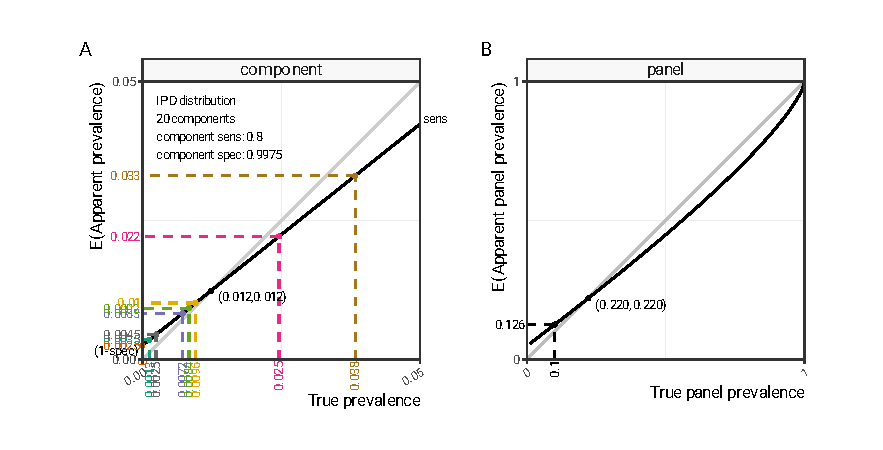
\includegraphics{fig/true-apparent-prevalence-component-panels.pdf}}
\caption{{\bf True versus apparent prevalence in multiplex test components and panel results.}
The apparent prevalence as a function of true prevalence in a simulated realistic scenario with excellent test specificity (99.75\%) and moderate test sensitivity (80\%). Panel A shows the individual component relationship and Panel B shows the panel relationship when 20 components are combined. Black lines show the relationship and the grey transparent lines are a guide to the eye showing perfect agreement. Note that subfigure A and B are on very different scales.
}
\label{fig3}
\end{figure}

In a synthetic but realistic scenario in Fig~\ref{fig3} (subfigure A), with excellent test specificity (99.75\%) and moderate test sensitivity (80\%), test positivity rate (apparent prevalence) is expected to be higher than true prevalence under a threshold of 1.2\% (subfigure A). When a set of 20 components are combined, that together result in a true panel prevalence of 10\%, the combined errors mean that the panel test positivity is higher than the true prevalence (subfigure B, dashed black lines). In Fig~\ref{fig1} and \nameref{S1_Appendix} we identify that false positives in one test balance out false positives in another test, and this makes panel test sensitivity a complex quantity that counter-intuitively depends on disease prevalence, component distribution, sensitivity and specificity. As a result the relationship between true panel prevalence and apparent panel prevalence (test positivity) is non-linear (Fig~\ref{fig3} subfigure B), and in this particular simulation test positivity will be an over-estimate of true prevalence, until true prevalence exceeds 22\%.

\begin{figure}[h!]
\centerline{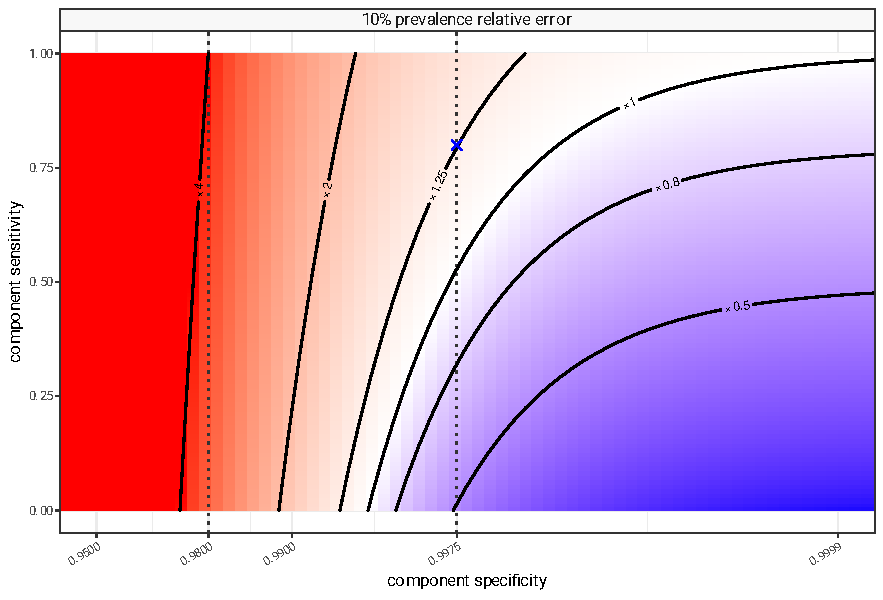
\includegraphics{fig/impact-error-by-sensitivity-specificity.pdf}}
\caption{{\bf Bias in apparent prevalence as an estimator for true prevalence.}
A simulated scenario of 20 components realistically distributed following patterns seen in IPD, with a simulated true prevalence of 10\%, and assuming a uniform sensitivity and a specificity for each of the component tests. Expected test positivity rates are calculated for all combinations of sensitivity and specificity, and compared to the true prevalence (10\%) as a ratio. At sensitivity of 80\% and specificity of 99.75\% (the blue cross) the test positivity rate will be about 1.26 times that of the true prevalence. Blue areas represent parameter space where test positivity is an underestimate of true prevalence due to excess false negatives, and red areas which test positivity is an overestimate due to excess false positives.}
\label{fig4}
\end{figure}

Component sensitivity and specificity determine the difference between true and apparent prevalence as shown in Fig~\ref{fig4}.  This shows the same scenario of 10\% prevalence, but shows the relative difference between true and apparent prevelance when varying sensitivity and specificity. The previous assumptions are marked as a blue cross in the figure, and at this high level of specificity (i.e. 99.75\% - right dotted vertical line in Fig~\ref{fig4}) the ratio between apparent and true prevalence is mostly influenced by test sensitivity. If we decrease sensitivity enough (to less than 50\%) eventually the false negative rate exceeds the combined false positive rate and apparent prevalence is smaller than true prevalence. In any situation where the specificity is lower, the balance of error is most influenced by test specificity, and test sensitivity becomes much less important as a factor determining the difference between true and apparent prevalence. Even marginally lower values of test specificity result in test positivity being a gross overestimate of panel prevalence. If the component test specificity is only 98\% (left dotted line) the combined 2\% false positive rate of 20 components is sufficient to drive the overall panel test positivity to 4 times the level of the true prevalence set in this simulation, regardless of the test sensitivity.

We have described that even low false positive rates in component tests lead to overestimates of uncommon components. The converse is true for components with comparatively high prevalence. In the scenario we have been using as an example, despite the excellent specificity of the tests and 10\% overall prevalence the balance of the component estimates is such that test positivity will overestimate true prevalence. This is seen more clearly in Fig~\ref{fig5} (left subfigure) in which simulated true prevalence levels (blue) are lower than test positivity (red) for all but two of the components (serotypes 3 and 8). In the right subfigure we see the effect of combining these into groups of 7, 13, 15 and 20 components, representing combinations of serotypes targeted by vaccines. As predicted, overestimates of prevalence are compounded and the size of each overestimate depends both on the number and distribution of the test components.

\begin{figure}[h!]
\centerline{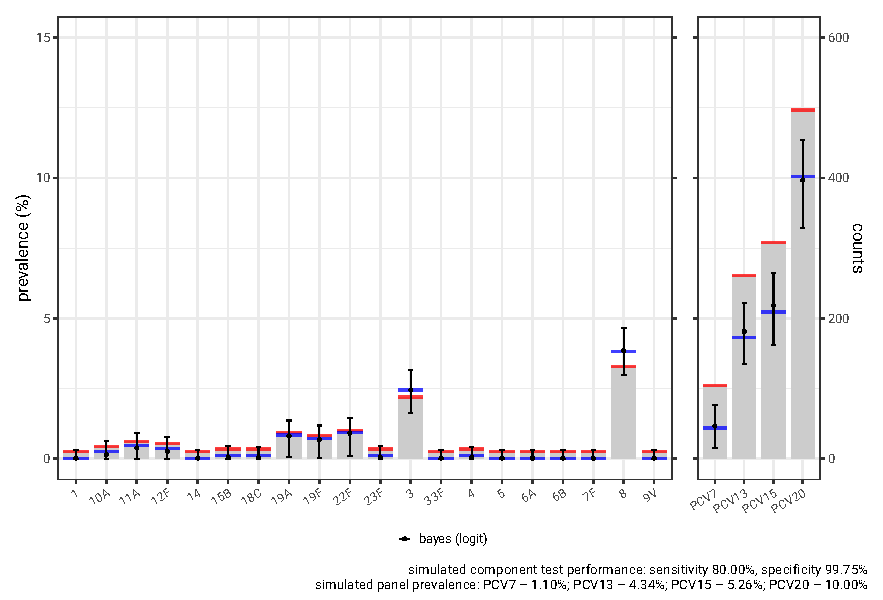
\includegraphics{fig/simulation_result_bayes_v2.pdf}}
\caption{{\bf Correction of bias in a single IPD scenario.}
The relative frequency of the 20 pneumococcal serotypes contained in PCV20, and identified in Bristol within the last 2 years, were converted to a distribution of 20 subtypes to give an overall PCV20 pneumococcal prevalence of 10\% (blue lines). Test positive samples were created assuming each serotype test had a sensitivity of 80\% and a specificity of 99.75\% (red lines) resulting in underestimates of true prevalence for serotypes 3 and 8, and overestimates for the remainder. The simulated test results for individual serotypes were aggregated into a PCV7 group (consisting of serotypes 4, 6B, 9V, 14, 18C, 19F, 23F), a PCV13 group (PCV7 groups plus 1, 3, 5, 6A, 7F, 19A), a PCV15 group (PCV13 plus 22F and 33F), and a PCV20 group (all serotypes). In the right subfigure combined test positivity for each group (apparent prevalence - red lines) overestimate true prevalence (blue line) for this scenario. We estimate true prevalence from test positivity, incorporating uncertainty in component sensitivity and specificity using a Bayesian model described in \nameref{S2_Appendix}. These estimates are shown as point estimates and 95\% credible intervals (black).}
\label{fig5}
\end{figure}

In \nameref{S2_Appendix} we describe methods for correcting this bias in both frequentist and Bayesian frameworks using results from the mathematical analysis (\nameref{S1_Appendix}). In Fig~\ref{fig5} the Bayesian correction is applied and we are able to correctly predict the true prevalence (blue) allowing for uncertainty in our knowledge of test sensitivity and specificity. This is examined in a broader range of scenarios in \nameref{S2_Appendix} but in summary both Bayesian and Lang-Reiczigel (frequentist) approaches work well when we have good prior information about the test sensitivity and specificity, but if these assumptions are very wrong, then we cannot expect either method to produce accurate estimates.

\section*{Discussion}

Combining multiplex test results into a panel commonly results in test positivity that significantly overestimates true prevalence. Multiplex testing simultaneously tests many hypotheses, and by combining the result into a single panel result leads to compounding of error. This error can be significant because of the low positive predictive value of individual component tests operating at low pre-test probability. This is critically dependent on component test specificity, and very high specificity is essential in tests which are designed to be interpreted as a combined result.

Panel test sensitivity is difficult to characterise. When multiplex tests are combined, components with a larger pre-test probability will generate more false negatives. In panel tests, false negative results in one component are over-ridden by any positives in other components. The specificity of the overall panel test is therefore a complicated function of component test sensitivity, specificity and pre-test probability (component prevalence), leading to higher panel sensitivity at higher prevalence. This is counter-intuitive as test sensitivity is usually regarded as independent of prevalence. This makes it very hard to compare panel test positivity rates in populations with different prevalence.

It remains possible to estimate true prevalence from test positivity, despite the complexities around panel test specificity and sensitivity. Positivity estimates generated by panel tests can be significantly biased and the expected value of test positivity is not a binomially distributed quantity so we cannot infer confidence intervals from an observation. The raw test positivity / apparent prevalence of a panel test is therefore very hard to interpret. We recommend use of the techniques described in this paper to produce modelled true prevalence estimates with confidence limits.

Sensitivity and specificity assumptions that incorporate uncertainty are critical in producing modelled true prevalence estimates. Specificity estimates for multiplex testing usually rely on a disease free control group, which may also be used to determine cut points to achieve set specificity levels, and can usually give us a reasonable estimate of component test specificity. Determining the sensitivity of the components of a multiplex test is much harder as it needs proven cases of disease with known subtype. These are difficult to find for rare disease subtypes, and gold standard identification of disease subtypes is not always available, or free from error\cite{loeffelholz2020,leber2018}. This results in a great deal of uncertainty in estimates of component test sensitivity. In some situations panel test sensitivity is estimated directly, however as we saw above panel test sensitivity is dependant on a range of factors including overall prevalence, and component distribution. Any direct estimates of panel sensitivity are not generalisable outside of the specific population tested. The methods presented here for modelling true prevalence from multiplex tests do allow for the uncertainty in sensitivity and specificity to be propagated. The accuracy of this correction however is dependent on the quality of the estimates of specificity and sensitivity (see \nameref{S2_Appendix}), complete mis-specification of either quantity prevents correct estimation of true prevalence. To improve accuracy and narrow the confidence intervals of estimates of prevalence it is far more important to characterise the sensitivity and specificity of the test than increase the sample size of testing. With a poorly understood test it is hard to draw any conclusions from the results.

The bias in panel test positivity is an inevitable consequence of combining multiple tests in environments with moderate to low prevalence. It can be prevented in a number of ways: either the specificity of the component tests must be increased, or second line confirmatory testing is performed, or the multiplex test can only be applied to populations with a very high overall disease prevalence. In the last case we may be able to use a multiplex test to determine which subtype of disease is causative if we already know the patient has the disease by using a different test, or using specific clinical diagnostic criteria that select patients with high probability of disease.

\section*{Conclusion}

The Biofire FilmArray\texttrademark respiratory panel 2.1 is one of a number of multiplex panels directed at respiratory pathogens\cite{ramanan2017}. It detects 19 viruses\cite{chang2022,loeffelholz2020} and has been relatively recently introduced in Bristol as a clinical test. A false positive for virus may result in conservative management of potentially treatable disease. Hence specificity of the viral components of the Biofire FilmArray\texttrademark multiplex test is important, as any false positives in the 19 viral components have to potential to influence therapy. There are multiple evaluations of the Biofire FilmArray\texttrademark panel\cite{popowitch2020,murphy2020,loeffelholz2020,leber2018,babady2013,chan2018} most of which compare different multiplex tests and are conducted using unwell patients to determine positive percent agreement between different panels. There has been less focus on a large scale evaluation of test specificity using disease free controls, and hence the risk of misclassification of a patient as having any of the 19 viral diseases in the panel is not well described. This is an area that could be improved, and using multiple comparisons in different populations it would be possible to use latent class approaches to infer component test parameters\cite{johnson2001}.

Uncertainty in test results due to lower sensitivity and specificity result in more noise at lower levels of prevalence\cite{haile2022,endo2020}. In vaccine effectivness studies using a test negative design this phenomenon acts to mask the effect of a vaccine in the lower prevalence vaccinated group. Hence test error always results in an underestimate of vaccine effectiveness\cite{endo2020}. The less sensitive the test, the greater this underestimate. For pneumococcal vaccination the serotype of pneumococcal disease is determined using two urine antigen detection (UAD) test panels\cite{pride2012,bonten2015} which together can identify 24 different pneumococcal serotypes. This is designed to be highly specific with individual serotype tests being around 99.75\%. Theory suggests that because of the issues identified here conclusions on vaccine effectiveness based on the UAD tests are most likely an underestimate \cite{endo2020}, however reuse of this panel test for determining disease burden is also affected. Despite excellent specificity, without correction, the large number of tests in the panel creates uncertainty in prevalence estimates using UAD tests, and difficulty in comparing results to those of other similar studies.

\section*{Supporting information}

% Include only the SI item label in the paragraph heading. Use the \nameref{label} command to cite SI items in the text.

\paragraph*{S1 Appendix.}
\label{S1_Appendix}
{\bf Sensitivity and specificity of combined panel tests.} Derivation of the performance metrics and true prevalence adjustments for combination tests.

\paragraph*{S2 Appendix.}
\label{S2_Appendix}
{\bf Propagation of uncertainty of combined panel tests.} Bayesian and frequentist approaches to estimating the uncertainty of panel test results.

\paragraph*{S3 R package.}
\label{S3_Github}
{\bf testerror: Uncertainty in Multiplex Panel Testing.}  Provides methods to support the estimation of epidemiological parameters based on the results of multiplex panel tests, doi:10.5281/zenodo.7691196. \url{https://bristol-vaccine-centre.github.io/testerror/}.


% \paragraph*{Supplementary 3.}
% \label{S3_Appendix}
% {\bf Additional figures.}

% \paragraph*{S1 Fig.}
% \label{S1_Fig}
% {\bf Bold the title sentence.} Add descriptive text after the title of the item (optional).

\section*{Acknowledgments}


\nolinenumbers

% Either type in your references using
% \begin{thebibliography}{}
% \bibitem{}
% Text
% \end{thebibliography}
%
% or
%
% Compile your BiBTeX database using our plos2015.bst
% style file and paste the contents of your .bbl file
% here. See http://journals.plos.org/plosone/s/latex for
% step-by-step instructions.
%
% \begin{thebibliography}{10}
%
% \bibitem{bib1}
% Conant GC, Wolfe KH.
% \newblock {{T}urning a hobby into a job: how duplicated genes find new
%   functions}.
% \newblock Nat Rev Genet. 2008 Dec;9(12):938--950.
%
% \bibitem{bib2}
% Ohno S.
% \newblock Evolution by gene duplication.
% \newblock London: George Alien \& Unwin Ltd. Berlin, Heidelberg and New York:
%   Springer-Verlag.; 1970.
%
% \bibitem{bib3}
% Magwire MM, Bayer F, Webster CL, Cao C, Jiggins FM.
% \newblock {{S}uccessive increases in the resistance of {D}rosophila to viral
%   infection through a transposon insertion followed by a {D}uplication}.
% \newblock PLoS Genet. 2011 Oct;7(10):e1002337.
%
%
%
% \end{thebibliography}

\bibliography{refs}


\end{document}

